\documentclass{standalone}
\usepackage{tikz}
\usetikzlibrary{matrix}

\begin{document}
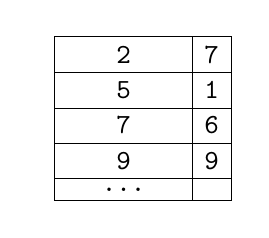
\begin{tikzpicture}
\matrix (m) [matrix of nodes,
nodes in empty cells,
nodes={font={\ttfamily}},
column sep=0,row sep=0,
column 1/.style={},
column 2/.style={nodes={text width=1.5cm,align=center}},
column 3/.style={nodes={minimum width=5mm}}
]{
&2&7\\
&5&1\\
&7&6\\
&9&9\\
&...&\\[1pt]
};

\draw (m-1-2.north west) rectangle (m-5-2.south east);
\draw (m-1-2.north east) rectangle (m-5-3.south east);


\foreach \x in {1,...,4} {
\draw (m-\x-2.south west) -- (m-\x-3.south east);
};
\end{tikzpicture}
\end{document}